\begin{figure} 
  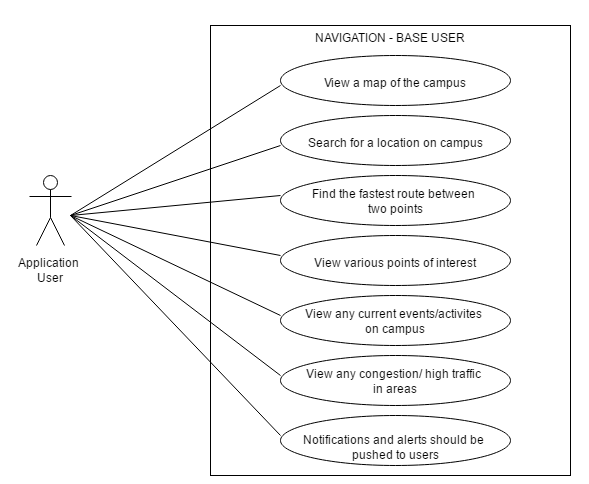
\includegraphics[width=\textwidth]{diagrams/Specific_Requirements/base_user_use_case.png}
\end{figure}
The base user requirements outlines the base/foundation functionality of the system. The inner workings of the system and it's subsystems will be expanded later in the document. Your typical base user will be able to do the following:
\\
\bigskip

\FuncReq
{View the map of campus}
{The user will be able to view the map through the use of the UI. The map itself will be saved on the system enabling access to it when connected or disconnected. It will contain all locations and venues located on campus itself.}
{TODO}
{TODO}
    \\
    \textbf{Actor system interaction model: View the map of campus }\\
    \begin{tabular}{ | p{6cm} | p{6cm} |}
    \hline
    Actor: Mobile User & System: NavUp \\ \hline
     & 0. The mobile app displays the main menu with the map and map info occupying most of the screen at the default position.\\ \hline
    1. The user scrolls around the map & 2. The app updates the map the map and map info that's in view, pulling information from the remote repository if needed and if possible.\\ \hline
    
    \end{tabular}
\\
\bigskip

\FuncReq
{Search for a location/venue on campus to be displayed on the map}
{The user needs to be able to search for a location/venue. This will involve a search bar (possible auto-complete functionality) where the user will enter the name of the location/venue. The mobile device will then search through it's database and indicate on the map when the location/venue has been found or display an appropriate prompt when the location/venue is not found.}
{TODO}
{TODO}
    \\
    \textbf{Actor system interaction model: Search for a location/venue on campus to be displayed on the map }\\
    \begin{tabular}{ | p{6cm} | p{6cm} |}
    \hline
    Actor: Mobile User & System: NavUp \\ \hline
    0. The user clicks on the magnification button & 1. The mobile app displays a menu to type in the location and venue.\\ \hline
    2. The user types in the location or venue & 3. Using information from cache and the remote repository, the app tries to perform autocomplete based on what the user is typing.\\ \hline
    4. The user chooses the autocomplete suggestion or types the search term out. & 5. The app generate a list of candidate locations/venues that match its internal cache or the remote repository.\\ \hline
    \end{tabular}
\\
\bigskip


\FuncReq
{Find the fastest route between two points}%This functional requirement will include finding the start point by gps or by manual input from the user
{
  \begin{enumerate}
    \item The user will be able to set the start point in the following ways:
      \begin{enumerate}
        \item By clicking on the map to indicate the start point or typing the name of the location into the search bar as described in another functional requirement. This should work for both online and offline.
        \item The start point is determined by integrating information from various sensors such as wifi and cellphone tower triangulation, gps, accelerometer and gyroscope. The functionality may work for both online and offline if possible.
      \end{enumerate}

    \item The user will be able to set the end point by tapping on the map to indicate the end point or typing the name of the location into the search bar as described in another functional requirement. This should work for both online and offline.
    \item After setting the start and end point the mobile app must calculate the fastest path between these two points and provide the directions to the user. If the device is offline it must make use of cached data to make an informed choice. If it is online, it must consult the remote repository for the most up to date congestion data.
  \end{enumerate}
  \mbox{}%enumerations cannot be ended with a newline
}
{TODO}
{TODO}
    \\
    \textbf{Actor system interaction model:Find the fastest route between two points }\\
    \begin{tabular}{ | p{6cm} | p{6cm} |}
    \hline
    Actor: Mobile User & System: NavUp \\ \hline
    0. The user clicks on the navigation button & 1. The mobile app displays a menu to type in the starting point and end point.\\ \hline
    2. The user selects the starting point by making a mark on the map or setting it as current location of the mobile device or searching for a place on the map & 3. If the mobile device is online, the remote server sends up to date congestion data to the mobile device. If the mobile device is offline, it uses cached data. In both cases the mobile phone calculate the fastest path using the congestion data, then displays the fastest path to the user.\\ \hline
    \end{tabular}
\\
\bigskip

\FuncReq
{View various points of interest}
{When selecting a certain building or location the mobile device should display information where applicable for the user to review. When offline the mobile device will use whatever it has in cache, if it is online it may consult the remote repository for the most up to date information.}
{TODO}
{TODO}
	\\
    \textbf{Actor system interaction model: View Various Points of Interest }\\
    \begin{tabular}{ | p{6cm} | p{6cm} |}
    \hline
    Actor: Mobile User & System: NavUp \\ \hline
    & 0. The mobile app displays a map of the campus.\\ \hline
    1. The user selects a destination & 2. The mobile application will display various points of interest along the path to the destination.\\ \hline
    \end{tabular}
\\
\bigskip
	\\
    \textbf{Actor system interaction model: View Various Points of Interest }\\
    \begin{tabular}{ | p{6cm} | p{6cm} |}
    \hline
    Actor: Mobile User & System: NavUp \\ \hline
    & 0. The mobile app displays a map of the campus.\\ \hline
    1. The user selects a location on the map & 2. The mobile application will display various points of interest in the surrounding areas.\\ \hline
    \end{tabular}
\\
\bigskip

\FuncReq
{View any current events or activities happening on campus}
{The mobile device should display various events and activities happening on campus on the current day as well as upcoming events and activities. When offline it should attempt to display activities and events that have not expired that resides in cache. When online, it should retrieve the most up to date list of events and activities from the remote repository.}
{TODO}
{TODO}
	\\
    \textbf{Actor system interaction model: View any current events or activities happening on campus }\\
    \begin{tabular}{ | p{6cm} | p{6cm} |}
    \hline
    Actor: Mobile User & System: NavUp \\ \hline
    & 0. The mobile app displays a map of the campus.\\ \hline
    1. The user selects a destination & 2. The mobile application will display various activities at venues along the way to the users destination.
    \\ \hline
    \end{tabular}
\\
	\\
    \textbf{Actor system interaction model: View any current events or activities happening on campus }\\
    \begin{tabular}{ | p{6cm} | p{6cm} |}
    \hline
    Actor: Mobile User & System: NavUp \\ \hline
    & 0. The mobile app displays a map of the campus.\\ \hline
    1. The user selects a location on the map & 2. The mobile application will display various activities at venues in and around the location selected.\\ \hline
    \end{tabular}
\\
\bigskip


\FuncReq
{Users should be able to view any congestion/ high traffic in areas}
{When using the application in a map view of the campus, users should be able to view the amount of pedestian traffic in surrounding areas. In addition to this any congestion in areas will also be indicated, this could be in the form of pedestrians or any other kind.}
{TODO}
{TODO}
\bigskip
	\\
    \textbf{Actor system interaction model: Users should be able to view any congestion/ high traffic in areas}\\
    \begin{tabular}{ | p{6cm} | p{6cm} |}
    \hline
    Actor: Mobile User & System: NavUp \\ \hline
    & 0. The mobile app displays a map of the campus.\\ \hline
    1. The user selects to view an indication of the pedestrian traffic and congestion on campus & 2. The mobile application will display various points at which there is high congestion and traffic.\\ \hline
    \end{tabular}
\\
\bigskip

\FuncReq
{View the map of campus}
{The user will be able to view the map through the use of the UI. The map itself will be saved on the system enabling access to it when connected or disconnected. It will contain all locations and venues located on campus itself.}
{TODO}
{TODO}
    \\
    \textbf{Actor system interaction model: View the map of campus }\\
    \begin{tabular}{ | p{6cm} | p{6cm} |}
    \hline
    Actor: Mobile User & System: NavUp \\ \hline
     & 0. The mobile app displays the main menu with the map and map info occupying most of the screen at the default position.\\ \hline
    1. The user scrolls around the map & 2. The app updates the map the map and map info that's in view, pulling information from the remote repository if needed and if possible.\\ \hline
    
    \end{tabular}
\\
\bigskip

\FuncReq
{Notifications and alerts should be pushed to users}
{The application will allow important notifications and alerts to be given to users in a mass instance. In emergency situations the application could be used to give users directions to assembly places or something of the like.}
{TODO}
{TODO}
